\documentclass[11pt]{article}
\usepackage{acl}
\usepackage{times}
\usepackage{latexsym}
\usepackage[T1]{fontenc}
\usepackage[utf8]{inputenc}
\usepackage{microtype}
\usepackage{graphicx}
\usepackage{booktabs}
\usepackage{amsmath}
\usepackage{amssymb}
\usepackage{tikz}
\usetikzlibrary{arrows.meta,positioning,shapes.geometric,calc,fit,backgrounds}
\usepackage{xcolor}
\usepackage{multirow}

\setcitestyle{numbers,square,comma}

\definecolor{nodeblue}{RGB}{60,90,160}
\definecolor{nodepurple}{RGB}{110,70,160}
\definecolor{edgegray}{RGB}{120,120,130}
\definecolor{lightbg}{RGB}{240,242,248}

\title{Asterism: A Hebbian-Weighted Knowledge Graph as a Priority Index over\\ Long-Term LLM Memory}

\author{Bidit Das \\
  Independent Researcher \\
  \texttt{github.com/biditdas18/asterism} \\}

\begin{document}
\maketitle

\begin{abstract}
Large language model (LLM) assistants increasingly persist user information across sessions as unstructured ``memory'' summaries. Such summaries behave like an unindexed heap: every stored fact carries equal retrieval priority, and nothing signals which facts currently matter most to the user. We present Asterism, a local-first system that builds a weighted, decaying knowledge graph from conversation history and injects a ranked subset of it into the model's context at inference time. The central design claim is architectural: the graph functions as a priority index over flat memory, in the same sense that a B-tree indexes an ordered file, with node weight acting as a salience signal analogous to an index key. We evaluate the mechanism across five retrieval conditions, two independently authored personal graphs, 100 priority queries per graph, and five assistant models spanning four vendors, with decoding held fixed and the graph reseeded before every call. We report three findings. First, the deployed system --- a weighted graph injected with a prioritization instruction --- increases \emph{decisiveness under ambiguity} over a flat list of the same facts: on priority-ranking queries scored with a pre-registered, held-out-validated commit/hedge metric, every model commits to a weight-justified answer more often under the weighted graph than under a flat list, in nearly every run. Second, this added decisiveness is \emph{more accurate} than flat memory in every model --- the graph conditions commit to the actually-highest-priority item more often than flat or no memory --- but we are explicit that absolute accuracy remains low: the best model identifies the true top priority only about 40\% of the time and most models far less, so the graph delivers a strong relative lift on a problem that is far from solved. Third, we isolate whether the benefit comes from the graph \emph{structure} or from the prioritization \emph{instruction} by testing a structure-only condition (the weighted graph with the instruction stripped): the structure-only effect is positive and run-consistent in nearly every model and graph, so the benefit is a property of the weighted structure itself and not merely of an instruction to prioritize. This generalizes a result that a smaller pilot had seen only in one model. We report the instrument's own reliability (scorer--human agreement $\kappa=0.64$, with errors that bias the measured gap toward the null), and two engineering components an automatically-populated index requires: an entity-resolution layer whose accuracy ceiling we measure, and a supersession mechanism that demotes contradicted facts. Local retrieval latency scales approximately linearly, near 34\,ms at 10{,}000 nodes. We release the full system, both benchmark graphs, and all negative results, and outline the direction they motivate: characterizing weight-structured, user-controllable, traceable memory as an alternative to similarity-based retrieval.
\end{abstract}

\section{Introduction}

Conversational LLM systems now routinely retain information about a user between sessions. The dominant form this retention takes is a running natural-language summary: a list of facts, preferences, and history that is prepended to the model's context on later turns. This format is simple and effective for recall, but it is structurally flat. Every fact sits at the same level. There is no representation of which facts are central to the user and which are incidental, no representation of how facts relate, and no representation of which facts have been superseded by newer ones.

In database terms, a flat memory summary is an \emph{unindexed heap}: a store you can scan but cannot query by priority. The contribution of this paper is to take that analogy literally and build the missing index. Asterism constructs a weighted directed graph from a user's conversation history, where nodes are concepts and entities, edges are relations, and edge and node weights encode how frequently and recently the user has engaged with each. At inference time, the highest-weight region of the graph is serialized into the model's context. The weight ordering is the index: it tells the retrieval step which facts to surface first, exactly as an index key tells a query planner where to look before touching the underlying data.

This framing makes a falsifiable prediction. If the graph is genuinely acting as a priority index and not merely as a memory store, then its benefit over an unstructured list of the same facts should appear specifically on tasks that require prioritization, and should largely vanish on tasks that require only recall. We test this directly, and we design the test to survive the obvious confounds. The deployed graph condition does two things at once: it imposes a weighted structure \emph{and} it instructs the model to prioritize high-weight nodes. A naive graph-versus-flat comparison cannot separate these. We therefore run five conditions against the same underlying facts: the weighted graph with its prioritization instruction (the deployed system), an unweighted flat list, no memory, a flat list that adds the prioritization \emph{instruction} without the structure, and a graph presented \emph{without} that instruction. The graph-versus-flat gap measures the deployed system's benefit; the last two conditions separate how much of that benefit is the structure and how much is the instruction. We hold decoding fixed, reseed the graph before every call so no response conditions on state a prior response wrote, and repeat the entire design across two independently authored personal graphs, one hundred priority queries per graph, and five assistant models spanning four vendors, five runs each.

We report three findings, each at its actual scope. First, the deployed system works across the board: on priority queries, the weighted-graph-plus-instruction condition produces more decisive commitment than a flat list of the same facts in every model we test, over two graphs and one hundred queries each, in nearly every run. Second, the added decisiveness is \emph{more accurate} than flat memory in every model --- committed answers land on the genuinely highest-priority item more often than under flat or no memory --- but we state the absolute levels plainly rather than only the relative lift: even the strongest model is correct only about 40\% of the time and most are well below that, so the graph improves priority routing without solving it. Third, and this is the result a smaller pilot got wrong for want of data, the benefit is a property of the graph \emph{structure} and not merely of the prioritization \emph{instruction}: a structure-only condition, with the instruction stripped, reproduces the effect in nearly every model and graph and holds run-to-run. At a pilot scale of twelve queries this structural effect looked confined to one model; at one hundred queries it generalizes across the panel. We prefer reporting the effect at this scope, with its low absolute ceiling and its one weak model stated openly, to a cleaner-sounding claim the data would not support.

Beyond the core comparison, an index over a live, automatically-populated store raises two engineering problems we treat as first-class and return to in Sections~\ref{sec:er} and~\ref{sec:temporal}: entity resolution (without which the graph fragments into near-duplicate nodes that corrupt the weight signal) and supersession (demoting facts a later turn contradicts, so a stale edge does not compete with the new one for retrieval).

Our contributions are:
\begin{enumerate}
  \item A framing of a weighted personal knowledge graph as a priority index over flat LLM memory, with node weight as the salience key (Section~\ref{sec:framing}).
  \item A five-condition evaluation across two independently authored graphs, one hundred priority queries per graph, and five models from four vendors, separating the deployed system's benefit from the value of memory per se and from the prioritization instruction. It shows the deployed system increases decisive commitment in every model, that the added decisiveness is more accurate than flat memory (though absolute accuracy stays low), and that the benefit is driven by the weighted structure itself, which reproduces the effect across nearly the whole panel (Section~\ref{sec:poc}).
  \item An empirical characterization of the entity-resolution ceiling for embedding-based canonicalization of short concept labels, including the negative result (Section~\ref{sec:er}).
  \item A supersession mechanism for demoting contradicted facts from retrieval, and a latency study showing approximately linear scaling to 10{,}000 nodes (Sections~\ref{sec:temporal},~\ref{sec:latency}).
\end{enumerate}

All code, benchmarks, and the seeded evaluation graph are publicly available.

\section{System Overview}
\label{sec:system}

Asterism is a local-first Python system. The entire graph lives in a single SQLite file on the user's machine; no data leaves the device except the user's own prompt and the injected context they choose to send to the model. Figure~\ref{fig:arch} shows the pipeline.

\begin{figure*}[t]
\centering
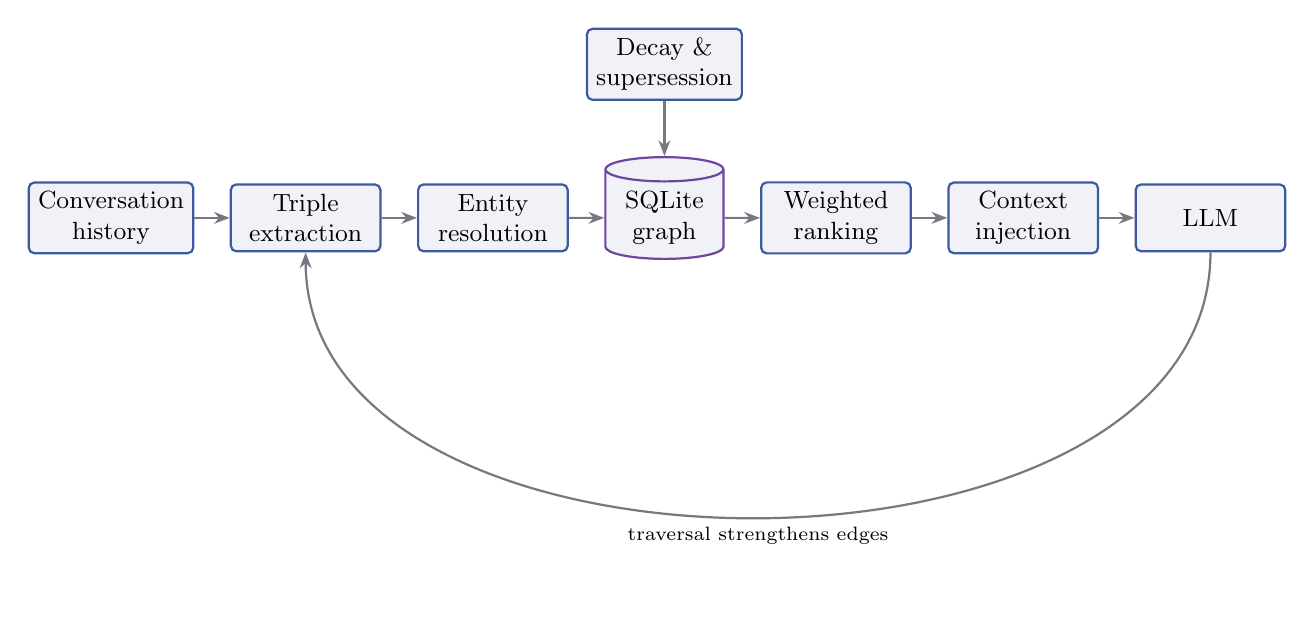
\begin{tikzpicture}[
  node distance=4.5mm,
  box/.style={rectangle, rounded corners=2pt, draw=nodeblue, thick, fill=lightbg, minimum height=8.5mm, minimum width=19mm, align=center, font=\small},
  store/.style={cylinder, shape border rotate=90, aspect=0.25, draw=nodepurple, thick, fill=lightbg, minimum height=11mm, minimum width=15mm, align=center, font=\small},
  arr/.style={-{Stealth[length=2mm]}, thick, draw=edgegray},
]
\node[box] (conv) {Conversation\\history};
\node[box, right=of conv] (extract) {Triple\\extraction};
\node[box, right=of extract] (resolve) {Entity\\resolution};
\node[store, right=of resolve] (db) {SQLite\\graph};
\node[box, above=7mm of db] (decay) {Decay \&\\supersession};
\node[box, right=of db] (rank) {Weighted\\ranking};
\node[box, right=of rank] (inject) {Context\\injection};
\node[box, right=of inject] (llm) {LLM};

\draw[arr] (conv) -- (extract);
\draw[arr] (extract) -- (resolve);
\draw[arr] (resolve) -- (db);
\draw[arr] (decay) -- (db);
\draw[arr] (db) -- (rank);
\draw[arr] (rank) -- (inject);
\draw[arr] (inject) -- (llm);
\draw[arr] (llm.south) to[out=-90,in=-90] node[below,font=\scriptsize,align=center] {traversal strengthens edges} (extract.south);

\end{tikzpicture}
\caption{Asterism pipeline. Conversation history is extracted into (source, relation, target) triples, canonicalized by entity resolution, and written to a local SQLite graph. A background process applies decay and supersession. At inference time the highest-weight subgraph is ranked and injected into the model's context. When the model traverses a relation in its response, the corresponding edge is strengthened, closing a Hebbian feedback loop.}
\label{fig:arch}
\end{figure*}

\paragraph{Extraction.} Each conversational exchange is processed by a small extraction model that emits (source, relation, target) triples. Sources and targets become nodes; relations become labeled, weighted edges.

\paragraph{Weighting and decay.} Every node and edge carries a scalar weight. Repeated engagement increases weight; disuse decreases it. Following the Hebbian principle that co-activated connections strengthen \citep{hebb1949organization}, an edge is reinforced whenever the model traverses it while answering a query. The complementary process is decay: an edge or node that accumulates session exposure without being traversed loses weight and is eventually pruned. Decay is measured in active session time rather than wall-clock time, so a concept does not fade while the user is simply away. This weight signal, accumulated over many sessions, is what the index ranks on.

\paragraph{Retrieval.} On each turn, the graph is queried for its highest-weight nodes and their relations, which are serialized into a compact block and placed in the model's system context. This is the read path of the index. We deliberately keep it simple: an ordered scan by weight, returning the top-$k$ nodes. Section~\ref{sec:latency} shows this is inexpensive even at ten thousand nodes.

\section{The Graph as a Priority Index}
\label{sec:framing}

The organizing idea of this work is that the structures a database uses to make an unindexed file queryable map directly onto the problem of making flat LLM memory prioritizable. We make the correspondence explicit because it drives the design and the evaluation.

A flat memory summary is a heap file: an append-only list of facts with no access structure. You can read all of it, but you cannot ask it ``what are the ten most important facts about this user'' without scanning everything and imposing an ordering after the fact. A B-tree \citep{bayer1972organization} solves the analogous problem for ordered files by maintaining a separate structure whose keys let a reader locate relevant records in logarithmic rather than linear cost. The key is not the data; it is a priority-ordered pointer into the data. In everyday terms, the difference is the index at the back of a book versus reading every page to find a topic: the index does not contain the book's content, but it tells you which pages matter and in what order to consult them.

Asterism's weighted graph plays the role of that index over the heap of conversational facts, with the following correspondences:

\begin{itemize}
  \item \textbf{Node weight $\leftrightarrow$ index key.} Weight is the quantity the retrieval step orders on. A high-weight node is a high-priority pointer: it is surfaced first, just as a B-tree directs a reader to the most relevant page before touching the file.
  \item \textbf{Graph traversal $\leftrightarrow$ query planning.} Answering a query by walking weighted relations is a plan over the memory space, in contrast to a full scan of the flat summary.
  \item \textbf{Decay $\leftrightarrow$ eviction policy.} Pruning low-weight, unused nodes is a cache-eviction discipline: it keeps the working index small and current, so retrieval priority reflects present rather than historical relevance.
  \item \textbf{Underlying facts persist.} Crucially, decaying a node removes it from the \emph{index}, not from the record of what was said. The distinction mirrors dropping an index entry without deleting the row.
\end{itemize}

We stress that graph-structured memory for LLMs is not itself new; systems such as Mem0 include graph-based memory representations \citep{chhikara2025mem0}, and MemGPT frames context management as an operating-system memory hierarchy \citep{packer2023memgpt}. Our claim is narrower and specific: that the \emph{weighting} of such a graph should be understood and evaluated as an index key, and that doing so predicts precisely where the structure helps. The next section tests that prediction.

\section{Core Evaluation: Index Structure versus Flat Recall}
\label{sec:poc}

\subsection{Design}

Evaluating a memory system risks conflating three different benefits: the benefit of having memory at all, the benefit of the particular structure imposed on it, and the benefit of instructing the model to act on that structure. The graph condition as deployed carries all three: it supplies facts, it imposes a weighted structure, and its system prompt instructs the model to prioritize high-weight nodes. To separate them, we run five conditions against the \emph{same underlying facts}:

\begin{enumerate}
  \item \textbf{Graph.} The top-weighted subgraph is injected, preserving weight ordering and relational structure, with an instruction to prioritize high-weight nodes (the deployed condition).
  \item \textbf{Flat list.} Every node label is injected as an unordered, unweighted list. The same facts are present; only the structure and salience signal are removed.
  \item \textbf{Flat list + instruction.} The same unordered list, but its prompt adds the same prioritize-and-commit instruction the graph carries, with no weights and no structure. This isolates the \emph{instruction}.
  \item \textbf{Graph, neutral.} The same weighted structure as \textsc{Graph}, but with the explicit prioritize/commit instruction removed and structure presented plainly. This isolates the \emph{structure}.
  \item \textbf{None.} No memory is injected.
\end{enumerate}

Two contrasts do the work. \textsc{Graph} vs.\ \textsc{Flat list} isolates structure-and-weighting from information content, since both see identical facts. \textsc{Graph, neutral} vs.\ \textsc{Flat list}, together with \textsc{Flat list + instruction} vs.\ \textsc{Flat list}, separates the effect of the structure from the effect of the instruction: if the effect is instructional, the instruction added to a flat list should reproduce it and the instruction-free graph should lose it; if it is structural, the reverse. \textsc{None} is a reference point.

We evaluate on two independently authored personal graphs of roughly fifty nodes each, organized into weighted domain/theme/concept chains. The two describe deliberately different users --- one an independent technical researcher, one a freelance designer with caregiving and family obligations --- with different domain mixes and different priority \emph{shapes}, so that a replication across both is evidence of generality rather than of one graph's idiosyncrasy. For each graph we focus the quantitative comparison on \emph{priority queries}: one hundred questions that ask what the user should focus on, what matters most, or which of two things to prioritize, each requiring the model to choose or rank rather than merely recall. The queries were generated by filling each graph's node labels into a fixed bank of question templates, and were frozen before any evaluation call; because the generator is templated and not one of the models under test, the query set cannot favor any model. For each query we derive the ground-truth highest-priority node from the seed weights, and flag as near-ties those whose top-two candidates fall within the decay step; these are excluded from the correctness metric only, since ``correct'' is ill-defined for them, but retained for the commit/hedge metric, which does not depend on ground truth.

To keep the comparison clean across a large call budget we fix three things. Decoding temperature is pinned to a single value on every backend, so cross-model differences cannot be attributed to sampling settings. The graph is reseeded from the pristine seed before \emph{every} individual call, so no response conditions on graph state that an earlier call's write-back mutated; an invariant check aborts a call rather than run it if the pre-call seed ever drifts. And we repeat the entire five-condition design across five assistant models spanning four vendors --- two Claude models (Sonnet and Opus class), one GPT model, one DeepSeek model, and one Kimi model --- with five independent runs each, reporting the mean over runs rather than a single draw. These five are all token-billed frontier models with no hard daily request caps, which is what makes a one-hundred-query campaign across five conditions and two graphs feasible. Earlier pilot runs also included two Gemini models and two free-tier open-weight models; the Gemini models' 250-request daily quota made a hundred-query campaign infeasible within the evaluation window, and the free-tier open-weight models both failed on throughput and on task comprehension (frequently naming the user node itself as the top priority). We therefore report the five token-billed models at full scale and exclude the others, disclosing this as a constraint of evaluating across vendors on consumer and free tiers. The graph-maintenance extractor is a separate, fixed model held constant across all conditions, so the assistant model is the only moving part.

\subsection{Metric}

We score each response with a single binary metric: does it \textsc{commit} to a specific ranked answer, or \textsc{hedge}? A response commits if it names a single top priority or makes an explicit choice and justifies it; it hedges if it defers the decision to the user, enumerates options without selecting, or answers ``it depends.'' The classifier is a deterministic rule, pre-registered and frozen before the evaluation run, and validated on a held-out set of eleven hand-labeled responses drawn from earlier development runs (not from the evaluation set), on which it achieved 11/11 agreement. We report the frozen classifier's output without post-hoc adjustment. Restricting the metric to priority queries is deliberate: commit-versus-hedge is only meaningful for questions that call for a ranking. Descriptive recall queries, for which a flat list is sufficient by construction, do not admit this metric and are excluded from it.

Because the entire dependent variable rests on this classifier, we validate it against human judgment on the actual evaluation data, not only the development set. One author independently labeled all 36 responses of one full run (twelve queries across the three core conditions) as commit or hedge without seeing the classifier's labels, and we computed agreement. Raw agreement was 83\% and Cohen's $\kappa$ was 0.64 (substantial). The disagreements are directional and, importantly, favor conservatism: of six disagreements, the classifier labeled as \textsc{hedge} four graph-condition responses a human read as commitments (for instance, a bare imperative ``Ship the package'' that the frozen rule's vocabulary did not cover), and over-credited two flat-list responses. Both directions understate the graph condition relative to the flat list, so the measured graph$-$flat gap is a conservative estimate of the true difference. We did not retune the classifier after seeing these disagreements; doing so would fit it to the evaluation data. The scorer--human comparison sheet is released with the code.

\subsection{Findings}

\begin{table*}[t]
\centering
\footnotesize
\setlength{\tabcolsep}{5pt}
\begin{tabular}{@{}llccccc|cc@{}}
\toprule
\textbf{Model} & \textbf{Gr} & \textbf{None} & \textbf{Flat} & \textbf{Fl+in} & \textbf{Graph} & \textbf{Gr,neut} & \textbf{G$-$F} & \textbf{Gn$-$F} \\
\midrule
Sonnet & G1 & 0.8 & 26.0 & 32.4 & 47.8 & 45.4 & +21.8 & +19.4 \\
Sonnet & G2 & 0.2 & 10.8 & 32.2 & 49.6 & 31.0 & +38.8 & +20.2 \\
Opus   & G1 & 1.0 & 13.2 & 30.8 & 49.2 & 36.8 & +36.0 & +23.6 \\
Opus   & G2 & 1.6 & 5.8 & 31.0 & 38.4 & 22.2 & +32.6 & +16.4 \\
GPT    & G1 & 23.6 & 35.6 & 40.4 & 50.8 & 40.8 & +15.2 & +5.2 \\
GPT    & G2 & 30.8 & 36.0 & 50.6 & 54.4 & 40.2 & +18.4 & +4.2 \\
DeepSeek & G1 & 5.0 & 10.6 & 17.4 & 15.0 & --- & +4.4 & --- \\
DeepSeek & G2 & 3.8 & 7.4 & 13.4 & 16.8 & 14.4 & +9.4 & +7.0 \\
Kimi   & G1 & 2.0 & 15.2 & 20.6 & 17.8 & 12.6 & +2.6 & $-$2.6 \\
Kimi   & G2 & 1.8 & 8.0 & 11.4 & 16.2 & 11.2 & +8.2 & +3.2 \\
\bottomrule
\end{tabular}
\caption{Mean commit rate (of 100 priority queries) over five runs, by model, graph, and condition, with the two key gaps at right: G$-$F = graph minus flat\_list (deployed benefit), Gn$-$F = graph\_neutral minus flat\_list (structure-only benefit). Decoding pinned, graph reseeded per call, all conditions scored by the same frozen held-out-validated classifier. \textsc{Fl+in} = flat list plus the prioritization instruction; \textsc{Gr,neut} = graph with the instruction removed. DeepSeek's G1 graph\_neutral cell is omitted: the model returned recurring empty responses in that condition (see text). Two free-tier models were separately excluded for throughput.}
\label{tab:commit}
\end{table*}

Table~\ref{tab:commit} reports the result across five models, two graphs, and one hundred queries per graph. We read it in three passes.

\paragraph{Finding 1: the deployed system increases decisiveness in every model.} Compare the \textsc{Graph} column (the weighted graph plus prioritization instruction, as deployed) to \textsc{Flat list} (the same facts, unweighted). The graph$-$flat gap (column G$-$F) is positive for all five models on both graphs, from $+2.6$ (Kimi G1) to $+38.8$ (Sonnet G2), and run-consistent (\textsc{Graph} $>$ \textsc{Flat list} in all five runs for most model--graph pairs, the weakest case being Kimi graph 1 at 3/5). \textsc{None} commits least throughout. Even GPT --- which at pilot scale committed at a high baseline that masked any structural benefit --- shows clear positive gaps here ($+15.2$, $+18.4$): with a larger, harder query set its no-memory rate is no longer a ceiling. The decisiveness benefit is not confined to models that hedge by default; it appears across the panel.

\paragraph{Finding 2: the decisiveness is more accurate than flat memory, but absolute accuracy is low.} A metric rewarding commitment could reward confident error. Because each seed graph has known weights, the correct top-priority item is defined, and we score correctness only on queries whose ground-truth weight separation exceeds the decay step; near-ties, where ``correct'' is not well defined, are excluded (leaving 96 of 100 scorable queries on graph 1 and 69 of 100 on graph 2, the latter graph having many near-ties by construction). We lead with the absolute numbers rather than the relative lift. Among scorable queries, the graph condition identifies the actually-highest-priority item in the following fractions: Sonnet 23\%/30\%, Opus 31\%/21\%, GPT 38\%/42\%, DeepSeek 9\%/10\%, Kimi 12\%/11\% (graph 1 / graph 2). So even the strongest model is correct on roughly four in ten priority queries, and most models on one to three in ten. Absolute priority routing is a hard, unsolved problem, and the weighted graph does not solve it. What it does is improve it: in every model and graph the graph condition is more often correct than the flat list (e.g.\ Sonnet 23\% vs.\ 8\%, Opus 31\% vs.\ 8\%, GPT 38\% vs.\ 18\%), so the added commitment is disproportionately correct commitment rather than confident noise. The finding is a real relative gain on top of a low absolute base, and we state both.

\paragraph{Finding 3: the benefit is structural, not merely instructional, and it generalizes.} Findings 1--2 concern the deployed system, which couples structure with instruction. We now ask which component carries the effect. \textsc{Graph, neutral} is the weighted structure with the prioritization instruction removed; if the benefit is structural it should survive (\textsc{Graph, neutral} $>$ \textsc{Flat list}). Column Gn$-$F reports this gap. It is positive in nine of the ten model--graph cells measured: Sonnet $+19.4/+20.2$, Opus $+23.6/+16.4$, GPT $+5.2/+4.2$, DeepSeek $+7.0$ (graph 2), Kimi $+3.2$ (graph 2). The structure-only effect holds run-to-run as well: graph\_neutral $>$ flat\_list in all five runs for Sonnet (both graphs), Opus (both), DeepSeek graph 2, and Kimi graph 2, and in 4/5 runs for GPT graph 2, with the deployed graph$>$flat likewise 5/5 for most pairs. The exceptions are honest and small: Kimi on graph 1 is the one negative cell ($-2.6$, structure-only in 2/5 runs), Kimi being the weakest and least consistent model in the panel, and DeepSeek's graph-1 structure-only cell is missing because that model returned recurring empty responses in that condition (discussed below). So stripping the instruction does \emph{not} remove the benefit: the weighted structure itself produces more decisive commitment, across nearly every model and graph we test. A twelve-query pilot had seen this structural effect clearly in only one model; at one hundred queries it generalizes across the panel, which we take as evidence that the pilot's apparent model-specificity was an artifact of scale rather than a real boundary.

Qualitatively, no-memory responses hedge honestly (``I don't have your priorities''), while flat-list responses, holding the same facts the graph does, hedge through filler and by reflecting the question back to the user; the graph's contribution is the salience signal that lets a model resolve the question rather than perform helpfulness around it.

We record one model-specific failure, because our guard against it is part of the method. DeepSeek, in the graph\_neutral condition on graph 1, repeatedly returned responses reporting normal completion yet containing no text while still consuming output tokens --- a silent empty-response failure. A universal guard that refuses to score empty or truncated content caught every instance and aborted the affected cell rather than recording a spurious hedge, so we report that cell as missing. The same guard caught an analogous failure in an earlier model during development. Detecting and excluding such outputs, rather than silently scoring them, is a necessary property of automated LLM evaluation.

\section{Entity Resolution and Its Ceiling}
\label{sec:er}

An index is only as good as the keys it orders. Because Asterism populates its graph automatically from extracted triples, the same real-world concept arrives under many surface forms across sessions. Without canonicalization, ``AI memory tools,'' ``AI memory tooling,'' and ``AI Memory Tools'' become three separate nodes, each accumulating a fraction of the weight the single underlying concept deserves. Fragmentation directly corrupts the index: it splits the salience signal and can prematurely decay a concept that is, in aggregate, highly active.

\subsection{Two-stage resolution}

We resolve labels at write time in two stages. First, a normalized exact/prefix match: labels are lowercased and whitespace-collapsed, and a new label matching or forming a normalized prefix of an existing one is merged. This is cheap and precise, and caught the clear duplicate variants in our live label set without error. Its ceiling is that it cannot merge meaning-equivalent variants that share no prefix, so a second stage falls through to embedding similarity, computing cosine similarity between label embeddings from a compact local model \citep{xiao2023cpack} and merging above a calibrated threshold. The model runs offline on CPU, on the write path only, so it does not affect retrieval latency.

\subsection{The measured ceiling}

The useful result is not that embedding resolution works but where it stops, which we measured against the live graph. The pattern held across every embedding model tested. Reworded or reordered labels that reuse the same vocabulary score high (0.92--0.98) and merge correctly: ``CLI Tools''/``CLI tool'' at 0.982, ``AI Memory Tools''/``AI memory tooling'' at 0.969. But \emph{true synonym substitution} --- different words for the same thing, e.g.\ ``LLM requires GPUs'' vs.\ ``Large Language Models need graphics processors'' --- scores only 0.745, in the same range as pairs that are merely topically related and must not merge (e.g.\ ``Philosophy \& Identity''/``Research Identity'' at 0.77--0.88), so no single threshold separates them. We calibrate to 0.92, below which false merges begin: this makes the resolver conservative, eliminating rewording-driven fragmentation (the common case) while declining to merge synonym pairs it cannot distinguish from distinct ones. The honest ceiling is more useful than an aggressive threshold that silently corrupts the graph; closing it properly needs supervision (a fine-tuned equivalence model or an LLM semantic check), which we leave to future work.

\section{Supersession: Demoting Contradicted Facts}
\label{sec:temporal}

An index over a live store must handle facts that change. When a user who ``uses Postgres'' switches to SQLite, naive decay eventually fades the old edge, but until it does both facts coexist and both can be retrieved as current, leaving a stale entry competing with a fresh one for a place in the injected context.

We add an explicit supersession mechanism scoped to the narrow, detectable case: a new edge from the same source, with the same relation, to a different target. On such a conflict the prior edge is marked superseded via a nullable self-reference and its time-to-live dropped so it becomes eligible for pruning; superseded edges are excluded from default injection, so the model sees only the current fact. A node is withheld only when \emph{every} fact-edge to it is superseded, so a concept with any live relation still appears. Superseded edges are not deleted --- they remain recoverable for explicit history queries (``what did I used to use''), preserving a distinction the flat summary cannot represent: a fact that is outdated versus one that was never true. The rule is deliberately conservative, avoiding open-ended contradiction detection that would risk demoting facts that only appear to conflict; the scoped version suffices to demonstrate the mechanism, demoting a predecessor from retrieval while leaving unrelated relations on the same source untouched.

\section{Latency and Scaling}
\label{sec:latency}

For the graph to serve as an index without harming interactive use, the read path must stay cheap as the graph grows. We benchmarked the retrieval step (loading and weight-ordering nodes and edges for injection) in isolation, excluding any model call, at three graph sizes over 20 runs each. Mean latency was 0.34\,ms at 102 nodes, 2.81\,ms at 1{,}006, and 33.87\,ms at 10{,}051 (P95 38.7\,ms): a roughly $99\times$ node increase yields a roughly $100\times$ latency increase, so retrieval scales approximately linearly and stays under 34\,ms even at ten thousand nodes, negligible beside the model call it precedes. The linear (not sub-linear) factor is a full-table weight ordering, reducible with a secondary index on the weight column. The supersession filter of Section~\ref{sec:temporal} adds 12--18\% to read latency (30.1 to 35.2\,ms at 10{,}051 nodes), a small cost of correctness well within the interactive budget.

\section{Related Work}
\label{sec:related}

\paragraph{LLM memory systems.} MemGPT frames context management as a virtual memory hierarchy, paging information between a limited context window and external storage under LLM control \citep{packer2023memgpt}. Mem0 provides a memory architecture that extracts and consolidates salient facts from conversation, including a graph-structured variant \citep{chhikara2025mem0}. Asterism shares the goal of persistent conversational memory but differs in emphasis: rather than optimizing recall or context-window management, it treats \emph{prioritization} as the core function and evaluates the weighted graph specifically as an index that supplies salience. Our five-condition comparison is designed to separate that prioritization benefit from the recall benefit those systems primarily target, and further to separate the structure from the instruction to use it.

\paragraph{Retrieval-augmented generation.} RAG retrieves passages by similarity to a query \citep{lewis2020retrieval}: it answers ``what is relevant to this query,'' whereas Asterism's weighting answers ``what is persistently important to this user,'' accumulated across sessions rather than computed per query. We take the empirical comparison between the two as the forward direction (Section~\ref{sec:conclusion}).

\paragraph{Indexing and biological memory.} The B-tree \citep{bayer1972organization} is the canonical priority-ordered access structure over a file too large to scan; we borrow its framing directly as a design and evaluation lever. The weighting dynamics draw on Hebbian plasticity, in which co-active connections strengthen \citep{hebb1949organization,shatz1992developing}, used as motivation for the traversal-strengthening rule, not a claim of biological fidelity.

\section{Conclusion}\label{sec:conclusion}

We presented Asterism, a local-first system that builds a weighted, decaying knowledge graph from conversation history and uses it as a priority index over flat LLM memory. Across five conditions, two authored graphs, one hundred queries per graph, and five models from four vendors, the results are consistent. The deployed weighted-graph-plus-instruction system increases decisive commitment over a flat list in every model, and that decisiveness is more accurate than flat memory in every model --- though absolute priority-routing accuracy stays low (near 40\% at best, often far less), so the graph improves a hard problem without solving it. Isolating structure from instruction, the structure-only condition reproduces the benefit in nearly every model and graph, so the effect is a property of the weighted structure itself, not merely of an instruction to prioritize; a smaller pilot had seen this in one model, and the scaled evaluation shows that apparent specificity was an artifact of scale. We also characterized entity resolution and supersession, showed retrieval scales approximately linearly to ten thousand nodes, and reported honestly the low absolute accuracies, the one weak model (Kimi), and a model-specific empty-response failure our guard caught and excluded.

The direction these results motivate is a comparison we do not frame as a contest. Similarity retrieval answers ``what is relevant to this query;'' a weighted, decaying graph answers ``what is persistently important to this user,'' with two properties retrieval does not inherently provide: a traceable, weight-grounded justification for why an item was surfaced, and direct user control over what is remembered. Whether this user-owned, auditable paradigm is a viable alternative to retrieval on prioritization tasks --- and whether its accuracy wins or loses against a strong retrieval baseline --- is worth answering either way: a negative result tells the field the graph path is not worth pursuing for accuracy; a positive one establishes structured personal memory as a genuine alternative. Characterizing that trade-off is where we take this next.

\section*{Limitations}

Our core metric is a single binary outcome (commit vs.\ hedge), scored over one hundred priority queries per graph, five models, and five runs each. This is a substantial sample, but the queries are templated variations on a fixed bank of prioritization phrasings, so they span the intended task without spanning the full range of ways real users express priority. Two graphs is better than one but is still not a population of users; the two were authored to differ in domain and priority shape, yet both were authored by us, and author-constructed personas may share latent structure a real user distribution would not.

Two limitations of the effect itself deserve emphasis. First, absolute accuracy is low: even the best model identifies the true top priority on only about 40\% of scorable queries, and most models on 10--30\%, so our claim is a relative improvement over flat memory, not a solved priority-routing problem. Second, while the structure-only effect generalizes across the panel, it is not uniform: Kimi is the weakest and least consistent model, showing the structural effect on graph 2 but not reliably on graph 1 (a negative gap there), and DeepSeek's graph-1 structure-only cell is missing entirely because that model returned recurring empty responses in that condition. So ``generalizes across nearly the whole panel'' is the honest scope, with one weak model and one missing cell stated openly. Our controls isolate structure from instruction but not the two components \emph{within} the structure: the weighted graph carries both a topology and explicit weight values, and we did not run a condition holding topology fixed while shuffling the weights, so we show structure matters, not whether the weights specifically or the graph shape carry it. Our panel also omits models we attempted but could not complete at this scale --- two Gemini models (daily-quota-limited) and two free-tier open-weight models (throughput and task-comprehension failures) --- which is a disclosed constraint of cross-vendor evaluation on consumer and free tiers.

Our controls isolate structure from instruction but not the two components \emph{within} the structure: the weighted graph carries both a topology (hierarchy, edges) and explicit weight values, and we did not run a condition holding topology fixed while removing or shuffling the weights. We show structure matters (in Sonnet), not whether the weights specifically or the graph shape carry it. We also do not compare end-task accuracy against a retrieval baseline such as RAG, or against external memory systems on a shared benchmark; the findings here are characterized behavioral effects on this setup, and the retrieval comparison is the forward direction outlined in the conclusion rather than a result we claim now. The entity-resolution ceiling is a limitation of the current unsupervised approach: true synonym pairs are not reliably merged and can still fragment the index. Supersession is scoped to the same-source/same-relation/different-target case and misses subtler contradictions. Because decay is measured in active-session rather than wall-clock time, decay topology depends on usage frequency: a daily user prunes old interests quickly while a sparse user's graph decays little in real time and can accumulate stale structure over a year. Latency, while linear and small, is measured on synthetic graphs and on retrieval alone; end-to-end latency is dominated by the model call. Finally, the system is single-user and local by design, and we have not studied multi-user or privacy-preserving extensions.

\section*{Ethics Statement}

Asterism is local-first: the graph is stored on the user's own device and no conversational data is transmitted except the user's prompt and the context they choose to inject into their model provider. Deleting the local store removes all derived data. The system infers user priorities from conversation history, and such inferences can be sensitive; because the data and index remain under the user's direct control and can be inspected or deleted, we regard the privacy surface as limited, but any deployment that centralized these graphs would raise concerns that the present design specifically avoids.

\section*{Declaration on Generative AI}

The authors used generative AI tools to assist with code for the system implementation and evaluation harness, and to support editing and refinement of the manuscript text (grammar, clarity, and structure). LLMs also appear as objects of study in the evaluation, as the assistant models being measured; those uses are described in the relevant sections. All research design, experimental decisions, analysis, and conclusions are the authors' own, and the authors reviewed and verified all content and take full responsibility for it.

\begin{thebibliography}{9}

\bibitem{hebb1949organization}
Donald O. Hebb. 1949.
\newblock \emph{The Organization of Behavior: A Neuropsychological Theory}.
\newblock Wiley, New York.

\bibitem{bayer1972organization}
Rudolf Bayer and Edward M. McCreight. 1972.
\newblock Organization and maintenance of large ordered indexes.
\newblock \emph{Acta Informatica}, 1(3):173--189.

\bibitem{chhikara2025mem0}
Prateek Chhikara, Dev Khant, Saket Aryan, Taranjeet Singh, and Deshraj Yadav. 2025.
\newblock Mem0: Building production-ready AI agents with scalable long-term memory.
\newblock \emph{arXiv preprint arXiv:2504.19413}.

\bibitem{packer2023memgpt}
Charles Packer, Vivian Fang, Shishir G. Patil, Kevin Lin, Sarah Wooders, and Joseph E. Gonzalez. 2023.
\newblock MemGPT: Towards LLMs as operating systems.
\newblock \emph{arXiv preprint arXiv:2310.08560}.

\bibitem{xiao2023cpack}
Shitao Xiao, Zheng Liu, Peitian Zhang, and Niklas Muennighoff. 2023.
\newblock C-Pack: Packaged resources to advance general Chinese embedding.
\newblock \emph{arXiv preprint arXiv:2309.07597}.

\bibitem{lewis2020retrieval}
Patrick Lewis, Ethan Perez, Aleksandra Piktus, Fabio Petroni, Vladimir Karpukhin, Naman Goyal, Heinrich K\"uttler, Mike Lewis, Wen-tau Yih, Tim Rockt\"aschel, Sebastian Riedel, and Douwe Kiela. 2020.
\newblock Retrieval-augmented generation for knowledge-intensive NLP tasks.
\newblock In \emph{Advances in Neural Information Processing Systems}, volume 33, pages 9459--9474.

\bibitem{shatz1992developing}
Carla J. Shatz. 1992.
\newblock The developing brain.
\newblock \emph{Scientific American}, 267(3):60--67.

\bibitem{hagberg2008exploring}
Aric A. Hagberg, Daniel A. Schult, and Pieter J. Swart. 2008.
\newblock Exploring network structure, dynamics, and function using NetworkX.
\newblock In \emph{Proceedings of the 7th Python in Science Conference (SciPy2008)}, pages 11--15, Pasadena, CA.

\end{thebibliography}

\appendix

\section{Reproducibility Details}
\label{app:repro}

The system is implemented in Python over SQLite, with the graph loaded into NetworkX \citep{hagberg2008exploring} for analysis. Triple extraction uses a small instruction-tuned model; entity-resolution embeddings use a compact local sentence-embedding model \citep{xiao2023cpack} producing 384-dimensional vectors, run offline on CPU. The evaluation graph, the five-condition comparison script and its multi-model runner, the latency benchmark, and the entity-resolution and supersession test suites are included in the public repository, together with the frozen scorer, the scorer--human agreement sheet, and all per-run results; reproduction instructions are in the repository README (\url{https://github.com/biditdas18/asterism}). Latency figures were produced by timing the retrieval function directly with a monotonic clock over 20 runs per scale, on synthetic graphs seeded with weighted domain/theme/concept chains; the real user database is never touched by the benchmark.

\end{document}
